\section{CLICpix}
Contact person: Dominik Dannheim (email: dominik.dannheim@cern.ch)
% \subsection{Collaborating Institutions}
% The vertex-detector R\&D for CLIC is carried out in the framework of the CLIC detector and physics
% collaboration (CLICdp), presently composed of 25 institutions~\cite{CLICdp-collaboration}.
% The main contributors to the vertex-detector
% project are
% Cambridge University,
% CERN,
% University of Geneva,
% Karlsruhe Institute of Technology (KIT),
% University of Liverpool,
% SLAC,
% Institute of Space Science Bucharest and the
% Spanish Network for Linear Colliders

\subsection{Introduction}
 The precision physics needs at the CLIC TeV-scale linear electron-positron collider
require a vertex-detector system with excellent flavour-tagging capabilities through
a measurement of displaced vertices in an environment with high rates
of beam-induced background events~\cite{Miyamoto:1425915}.
As a result, the CLIC vertex-detector system needs to have excellent spatial resolution
(\unit[3]{\micron}),
full geometrical coverage extending to low polar angles, extremely low material budget
(0.2\% $X_0$ per layer),
low occupancy facilitated by time-tagging (\unit[10]{ns} precision), and sufficient heat
removal from sensors and readout.
A concept based on hybrid pixel-detector technology is under development
for the CLIC vertex detector. It comprises fast, low-power and small-pitch readout
ASICs implemented in \unit[65]{nm} CMOS technology (CLICpix) coupled to ultra-thin planar sensors
or active HV-CMOS sensors via low-mass interconnects. The power dissipation of the
readout chips is reduced by means of power pulsing, allowing for a cooling system
based on forced gas flow. Through-Silicon Via (TSV) vertical interconnects remove the need for wire
bonding connections on the side of the readout ASICs
and therefore allow for an efficient tiling to form larger modules with minimal
inactive areas.

\begin{figure}
    \centering
    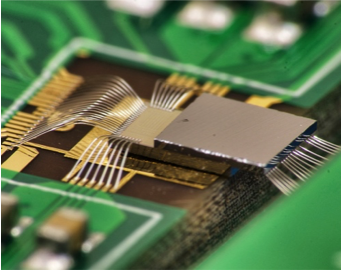
\includegraphics[width=.4\textwidth]{VertexDetector/CLICPix/ccpdv3_clicpix.png}
    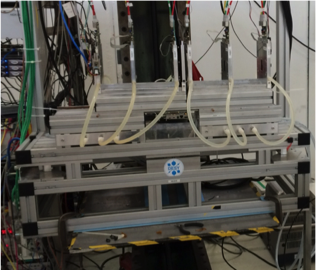
\includegraphics[width=.4\textwidth]{VertexDetector/CLICPix/timepix3_telescope.png}
    \caption{Left:CCPDv3 + CLICPix. Right: Timepix3 in the AIDA telescope (CERN PS-T9)}
    \label{fig:VertexDetector:clicpix}
\end{figure}
\subsection{Recent Milestones}
A broad hardware R\&D program is in place, addressing the challenges for the CLIC
vertex detector in an integrated approach~\cite{1748-0221-10-03-C03025}. Recent achievements
in the sensor and readout domain include:
\begin{description}
\item[Hybrid pixel assemblies with ultra-thin planar sensors]
Planar pixel sensors with \unit[55]{\micron} pitch and different thicknesses (\unit[50--300]{\micron})
were procured from different vendors and bump-bonded to Timepix~\cite{Llopart2007485} readout
ASICs (100 and \unit[700]{\micron} thickness).
Slim-edge sensor designs are compared to designs
with active edges.
Preliminary beam-test results show very good efficiencies in both cases, extending beyond the
edge pixels~\cite{Redford:1966932}.
For \unit[50]{\micron} sensor thickness and nominal readout parameters, the fraction of multi-pixel clusters
is approximately 20\%.
Single-point resolutions of approximately \unit[3]{\micron} have been extracted
for clusters of two pixels using charge interpolation and taking into account
non-linear charge sharing.
\item[CLICpix demonstrator ASIC]
A CLICpix demonstrator chip has been produced in \unit[65]{nm} CMOS technology,
including a $64 \times 64$ pixel matrix and power-pulsing capability~\cite{Valerio:1507691}.
The pixel size is $\unit[25]{\micron}\times\unit[25]{\micron}$. Simultaneous
4-bit Time-Of-Arrival (ToA) and Time-Over-Threshold (ToT) measurements
are implemented in each pixel, allowing for a front-end time slicing
with approximately \unit[10]{ns} and for measuring the charge
to improve the position resolution through interpolation.
The full chip can be read out in less than
$\unit[800]{\upmu s}$ (for 10\% occupancy), using a \unit[320]{MHz} readout clock and zero suppression.
The
power consumption of the chip is dominated by the analog frontend
with a peak power corresponding to $\unit[2]{W/cm^2}$. The total average power
consumption can be reduced to a value below the target of $\unit[50]{mW/cm^2}$
by means of power gating for the analog part and clock gating for the digital part.
Readout tests have confirmed that the CLICpix demonstrator chip
is fully functional and the power consumption and performance are in agreement with
simulations~\cite{Valerio:1635171}.
Hybrid modules of CLICpix ASICs with planar slim-edge
sensor prototypes are currently in production.
\item[Capacitively coupled active HV-CMOS sensors]
Hybrid assemblies of CLICpix prototype chips with CCPDv3 active sensors
have been produced and tested.
The sensors are implemented in
a \unit[180]{nm} high-voltage CMOS process~\cite{Peric2013131}. A deep n-well above the low-resistivity
(few $\Omega$cm) p substrate
surrounds low-voltage p-wells and acts as the signal collecting electrode.
A nominal operation voltage of -\unit[60]{V} at the
n-well results in a depletion layer of approximately \unit[10--20]{\micron} in the p substrate.
 The fast drift signal collected in this
depletion layer passes through a two-stage transimpedance
amplifier in each pixel and the resulting voltage signal is capacitively coupled to the CLICpix
ASIC through a layer of glue a few microns thick.
Laboratory tests with radioactive sources show a good signal-to-noise performance for the
active sensor output. Preliminary test-beam results with CLICpix-CCPDv3 assemblies suggest a
detection efficiency of $>99\%$ for minimum ionising particles and a high fraction of
single-pixel clusters with a position resolution of
approximately \unit[7]{\micron}, as expected for \unit[25]{\micron} pixel pitch.
\item[Through Silicon Vias (TSV)]
A ``via last'' TSV process developed in collaboration with
CEA-LETI has demonstrated the feasibility of TSVs on functional
readout ASICs from the Medipix/Timepix chip family~\cite{6575630}.
The project uses Medipix3 readout wafers produced in \unit[130]{nm} CMOS
technology. The wafers are thinned to \unit[120]{\micron} and the resulting vias
have a diameter of \unit[60]{\micron}.
An ongoing  continuation of the TSV project aims at producing
TSVs in Timepix3 ASIC wafers thinned to \unit[50]{\micron}.
\end{description}
\subsection{Engineering Challenges}
The detector performance requirements lead to challenging constraints
for the mechanical and electrical integration of the vertex-detector
components and its cooling system. An integrated approach is followed,
addressing several of the critical R\&D issues in these domains:
\begin{description}
\item[Power delivery and power pulsing] A low-mass power-pulsing and power-delivery
system optimised for the small duty cycle of the CLIC machine has been
developed~\cite{1748-0221-8-01-C01057}. Controlled current sources
deliver a low and almost constant current ($<\unit[300]{mA}$ per ladder)
into the vertex region through low-mass cables. The energy needed by the readout ASICs during the time of the collisions
and detector readout is stored locally in silicon capacitors. Low-dropout regulators provide the necessary stability
of the output voltage for the analog ($\Delta V\approx16$mV) and the digital part
($\Delta V\approx\unit[70]{mV}$) of the readout ASICs.
Prototypes have been tested successfully with dummy loads emulating the power consumption
of the 12 readout ASICs in a half ladder. The total contribution of the
powering infrastructure to the material budget of each barrel layer is
approximately 0.1\%X$_0$. It is expected to decrease to less than $0.05\%$X$_0$ with evolving silicon-capacitor technology.
\item[Cooling] Even with power pulsing a total power of approximately \unit[500]{W} will be dissipated in the vertex detectors alone. To limit the amount of material in the vertex-detector region, a cooling
system based on forced air flow is under development~\cite{DuarteRamos:1572989}. Finite-element Computational Fluid Dynamics (CFD) simulations show that air cooling is feasible. For a mass flow of \unit[20]{g/s}, the temperature increase
in the vertex detector is limited to approximately \unit[40]{\textdegree C}. The proposed cooling scheme is being
validated in thermal mockups. Preliminary results confirm the validity of the simulations.
\item[Mechanical supports] The low overall material budget leaves only about 0.05\%X$_0$ per
detection layer for mechanical supports. Prototypes based on Carbon-Fibre-Reinforced Polymers
(CFRP) are under study~\cite{VillarejoBermudez:1982810}. Bending-stiffness calculations have been validated in
finite-element simulations
and with bending tests. Measurements within an air-cooling mockup show
that the air-flow induced vibrations are at an acceptable level of approximately $\unit[1-2]{\micron}$ RMS
amplitude for the direction perpendicular to the detector plane and at nominal flow conditions.
\item[Assembly and access scenarios]
Assembly and access scenarios for in-situ testing have been developed,
taking into account the constraints from the surrounding detector elements~\cite{VillarejoBermudez:1982810}.
Realistic cabling layouts are proposed and evaluated in terms of their impact on the
global and local material budget.
\end{description}
\subsection{Future Plans}
The technical development programme for the CLIC vertex detector aims at building
demonstration modules for the main components of the vertex detector system
in time for the next update of the European Strategy
for Particle Physics in 2018/19. To reach this medium-term goal, several technology prototypes
are under development.
Ultra-thin edgeless hybrid pixel assemblies with Timepix3 readout ASICs (including ASICs thinned to \unit[50]{\micron}
and processed with TSVs) are currently in production.
The next version of the CLICpix demonstrator
ASIC (CLICpix2) is foreseen to be produced in the second half of 2015. It contains a larger
pixel matrix ($128\times 128$) and higher dynamic range (8-bit ToA and 5-bit ToT).
Slim-edge and edgeless sensors matching the $128\times 128$ CLICpix2 footprint have already been produced and an
improved version of the CCPD active HV-CMOS sensor will be submitted for production by the end of 2015.
